\documentclass[10pt,mathserif]{beamer}

\usepackage{graphicx,amsmath,amssymb,tikz,psfrag,pifont,amssymb}
\input defs.tex

%% formatting

\mode<presentation>
{
  \usetheme{default}
}
\setbeamertemplate{navigation symbols}{}
\usecolortheme[rgb={0.13,0.28,0.59}]{structure}
\setbeamertemplate{itemize subitem}{--}
\setbeamertemplate{frametitle} {
  \begin{center}
    {\large\bf \insertframetitle}
  \end{center}
}

\newcommand{\cmark}{\ding{51}}
\newcommand{\xmark}{\ding{55}}

\newcommand\footlineon{
  \setbeamertemplate{footline} {
    \begin{beamercolorbox}[ht=2.5ex,dp=1.125ex,leftskip=.8cm,rightskip=.6cm]{structure}
      \footnotesize \insertsection
      \hfill
      {\insertframenumber}
    \end{beamercolorbox}
    \vskip 0.45cm
  }
}
\footlineon

\AtBeginSection[]
{
  \begin{frame}<beamer>
    \frametitle{Outline}
    \tableofcontents[currentsection,currentsubsection]
  \end{frame}
}

%% begin presentation

\title{\large \bfseries Recent Results in Web Security \\ Content
  Sniffing Attacks, Insider Attacks, and Botnet
  Detection}

\author{Conrad Stansbury and Dennis Wang\\[3ex]
  Stanford University}

\date{December 1, 2014}

\begin{document}

\frame{
  \thispagestyle{empty}
  \titlepage
}


\section{State of Web Security}

\begin{frame}
  \frametitle{Attacks Originating Outside the Network}
  \begin{block}{State of the Art}
    \begin{itemize}
    \item We have seen many techniques exist in ML for intruder
      detection
    \item Hybridized schemes allow the construction of strong IDS/IPS
      with acceptable FP rates
    \item High stakes game means lots of research (from the perspective
      of both detection and anti-detection advocates!)
    \end{itemize}
  \end{block}

  \begin{block}{Challenges}
    \begin{itemize}
    \item Security is largely a reactionary field
    \item Intruders just have to evade whatever particular defenses are
      in use at their target
    \item In many cases, intruders just have to make their traffic look
      like typical traffic to get by, and there is a wide diversity of
      types of traffic and flow patterns
    \end{itemize}
  \end{block}
\end{frame}

\begin{frame}
  \frametitle{Attacks Originating Inside the Network}
  \begin{block}{State of the Art}
    \begin{itemize}
    \item Signature based schemes as well as anomaly detection schemes
    \item Today we will see a hybridized scheme that successfully
      bridges gaps in signature and models and HMMs
    \end{itemize}
  \end{block}

  \begin{block}{Challenges}
    \begin{itemize}
    \item More and more attacks are insider attacks
    \item Difficult to defend because insiders often have increased
      privileges relative to outside connections--established trust
    \item Most security techniques defend against inbound traffic
      \begin{itemize}
      \item High volume of attack from exterior
      \item Unwanted disturbances of workflow not well tolerated
      \end{itemize}
    \end{itemize}
  \end{block}
\end{frame}

\section{Server Side Content Sniffing Detection}

\begin{frame}
  \frametitle{Background}
  \begin{block}{Content Sniffing Attacks}
  \end{block}
\end{frame}
\begin{frame}
  \frametitle{The Problem}
  \begin{block}{Current Detection Method}
  \end{block}
  \begin{block}{Limitations}
  \end{block}
\end{frame}
\begin{frame}
  \frametitle{Detection Scheme Overview}
  \begin{block}{Detection Steps}
  \end{block}
\end{frame}
\begin{frame}
  \frametitle{Detection Scheme Flow}
  \begin{block}{Detection Steps}
  % picture
  \end{block}
\end{frame}

\section{Hybrid Schemes for Insider Attack Detection}

\begin{frame}
  \frametitle{Inspiration}
  \begin{block}{Signature-Based Detection}
  \end{block}
  \begin{block}{Anomaly-Based Detection}
  \end{block}
\end{frame}
\begin{frame}
  \frametitle{Insider vs. Intruder Attack}
  \begin{block}{Intruder Attack}
  \end{block}
  \begin{block}{Insider Attack}
  \end{block}
\end{frame}
\begin{frame}
  \frametitle{Detection Scheme Overview}
  \begin{block}{Detection Steps}
  \end{block}
\end{frame}
\begin{frame}
  \frametitle{Detection Scheme Flow}
  \begin{block}{Detection Steps}
  % picture
  \end{block}
\end{frame}

\section{Differentiating Botnets from Flash Crowds}
\begin{frame}
  \frametitle{The Problem}
  \begin{block}{Detecting Botnets in Light of Similar Signals}
    \begin{itemize}
    \item Flagging malicious traffic on the basis of volume is
      insufficient
    \item Legitimate traffic often spikes as a result of world events
      \begin{itemize}
      \item World events
      \item Link aggregators and ``virality''
      \end{itemize}
    \item If we can't separate attack traffic from these natural surges
      we can't stop DDoS--blocking real traffic is a DoS
    \end{itemize}
  \end{block}
  \begin{block}{Anti-detection}
    \begin{itemize}
    \item Attackers would like to disguise their traffic by making it
      look like a flash crowd
    \item Flash crowd aware systems might accept attack traffic if it is
      sufficiently similar
    \end{itemize}
  \end{block}
\end{frame}

\begin{frame}
  \frametitle{Differing Signatures Between Botnets and Flash Crowds}
  \begin{block}{Key Observation}
    \begin{itemize}
    \item Studies indicate that attack tools/dispatch scripts are
      homogeneous inside a single botnet
    \item Fewer bots than real users
    \item If an aggregate attack flow is composed of attack flows from
      many similar bots, it has a similar flow standard deviation to that of one
      bot
    \item We should expect that attack traffic has low standard deviation
    \end{itemize}
  \end{block}
\end{frame}

\begin{frame}
  \frametitle{Differing Signatures Between Botnets and Flash Crowds}
  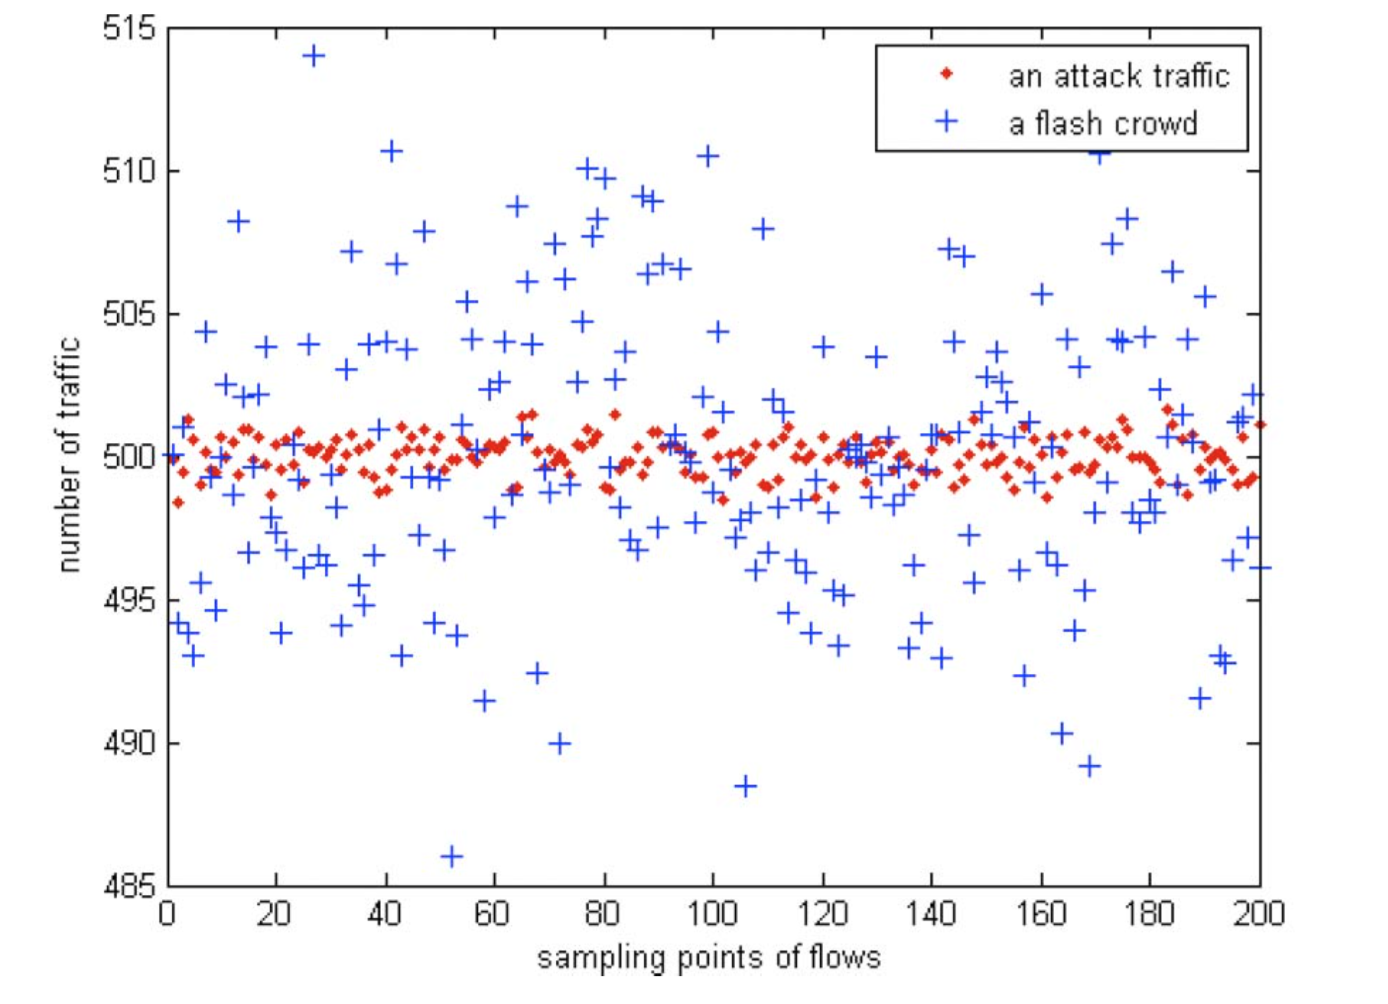
\includegraphics[width=\textwidth,natwidth=1388,natheight=1004]{figures/traffic_comp.png}
\end{frame}

\begin{frame}
  \frametitle{Detection Scheme Overview}
  \begin{columns}[T]
    \begin{column}{0.5\textwidth}
      \begin{block}{What is a flow?}
        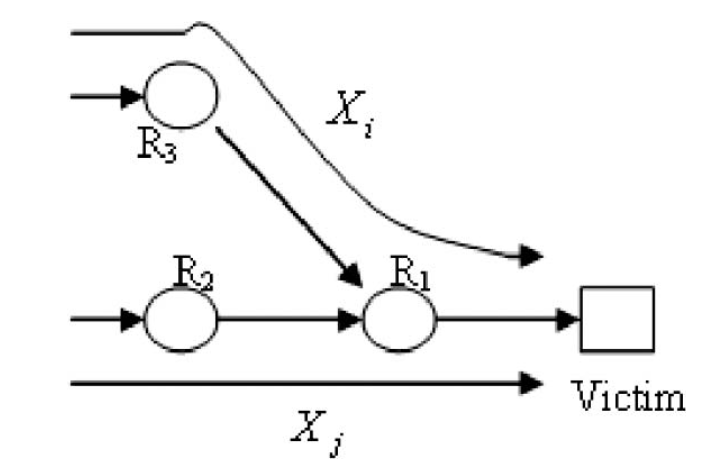
\includegraphics[width=\textwidth,natwidth=714,natheight=472]{figures/flow.png}
      \end{block}
      \vspace{-0.2cm}
      \begin{center}
      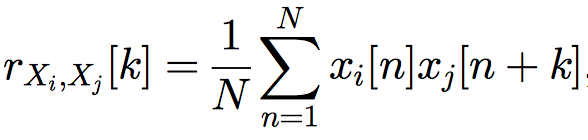
\includegraphics[width=0.7\textwidth,natwidth=558,natheight=140]{figures/correlation_def.png}
      \vspace{-0.01cm}
      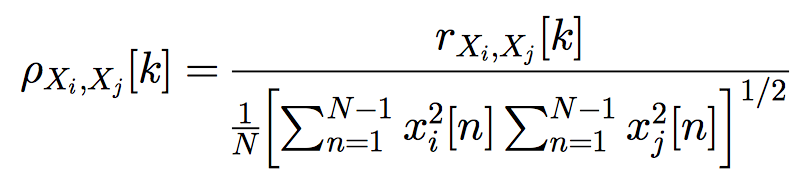
\includegraphics[width=\textwidth,natwidth=798,natheight=188]{figures/correlation_coeff_def.png}
    \end{center}
    \end{column}
    \begin{column}{0.5\textwidth}
      \begin{block}{Exploit Flow Correlations}
        \begin{itemize}
          \item Flow is network exterior node traffic to a particular
            destination
          \item Compute pairwise correlation of discretized flow for
            different offsets of the flow vectors
          \item Choose correlation to be maximum among these
          \item Similarity measure: correlation coefficient
        \end{itemize}
      \end{block}

    \end{column}
  \end{columns}
\end{frame}

\begin{frame}
  \frametitle{Detection Scheme Overview}
  \begin{block}{Correlation Coeffient Cutoff for IDing Traffic}
    \begin{itemize}
      \item Following premise that botnet traffic has higher correlation
        coefficient, choose some cutoff parameter $\delta$
      \item Correlation at nodes $i,j$ flagged as malicious
        ($I_{X_i,X_j} = 1$) if
        \[\max_k(\rho_{X_i,X_j}\left[ k \right]) > \delta\]
        not malicious ($I_{X_i,X_j} = 0$) otherwise
      \item Another independent parameter $\delta'$ is used to
        determine whether an attack is ongoing based on the $I$'s
      \item Being attacked when
        \[\frac{\sum_{i\neq j}I_{X_i,X_j}}{\binom{M}{2}} > \delta'\]
    \end{itemize}
  \end{block}
\end{frame}

\begin{frame}
  \frametitle{Results: World Cup}
  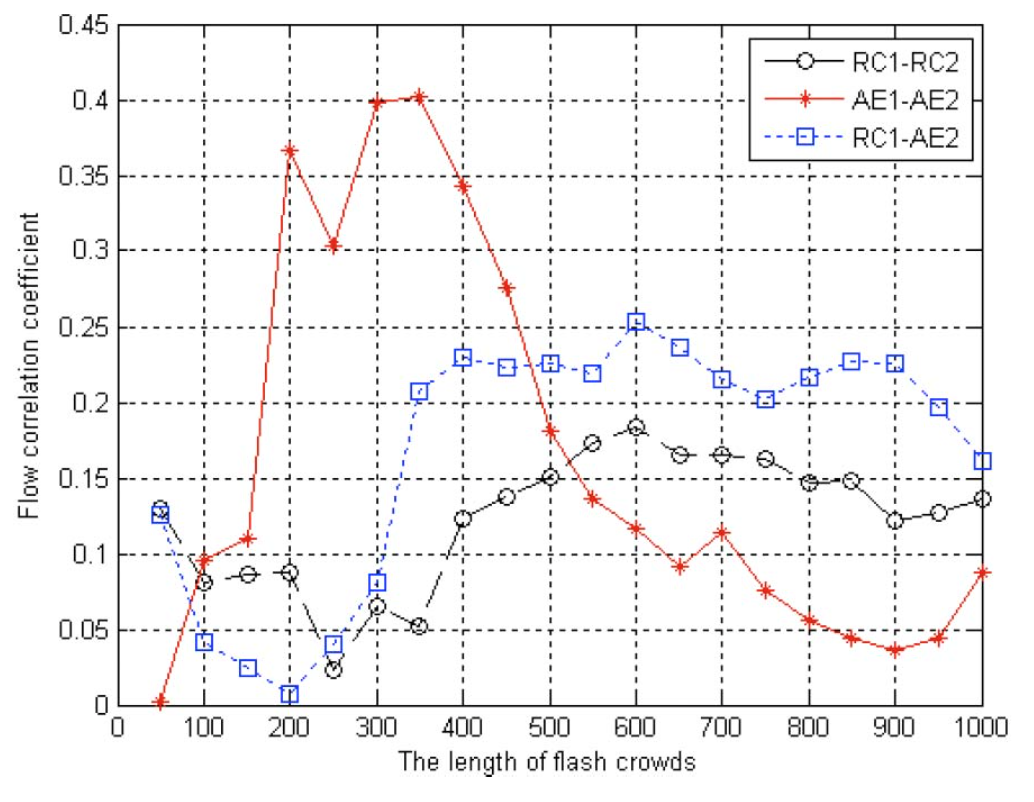
\includegraphics[width=0.9\textwidth,natwidth=1034,natheight=802]{figures/world_cup.png}
\end{frame}

\begin{frame}
  \frametitle{Results: General Flash Crowds}
  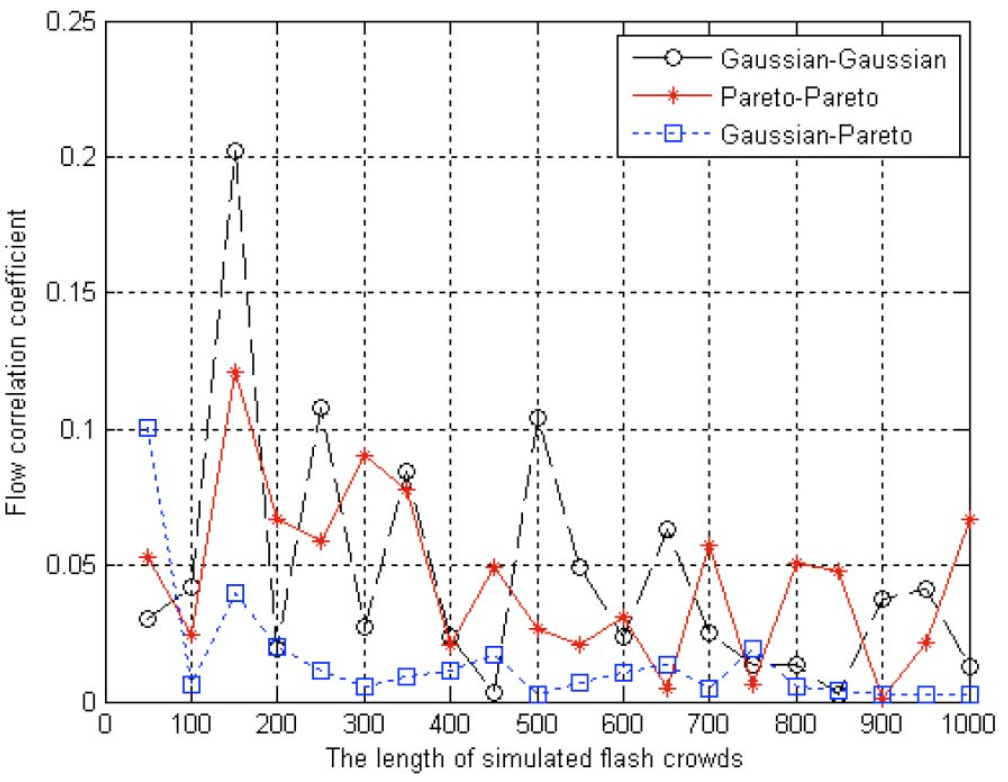
\includegraphics[width=0.9\textwidth,natwidth=1008,natheight=782]{figures/gen_flash_crowds.png}
\end{frame}

\begin{frame}
  \frametitle{Results: Attacks with Delays}
  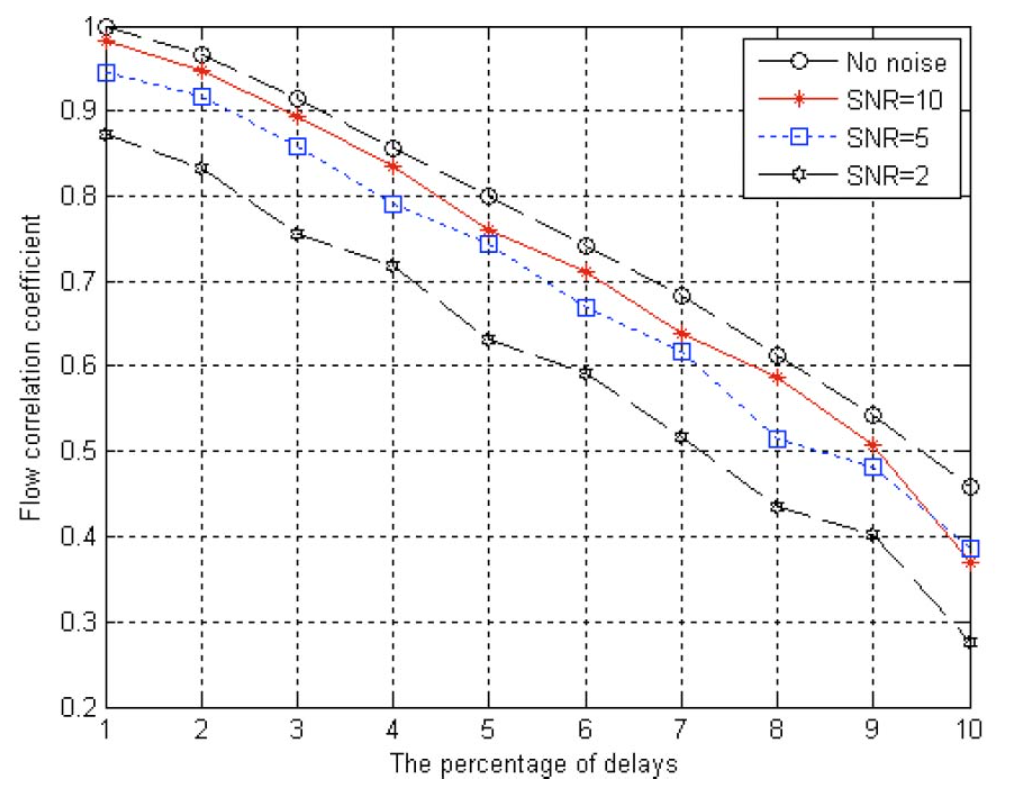
\includegraphics[width=0.9\textwidth,natwidth=1012,natheight=796]{figures/attack_delay.png}
\end{frame}

\begin{frame}
  \frametitle{Results: Aggregate Attack Merging}
  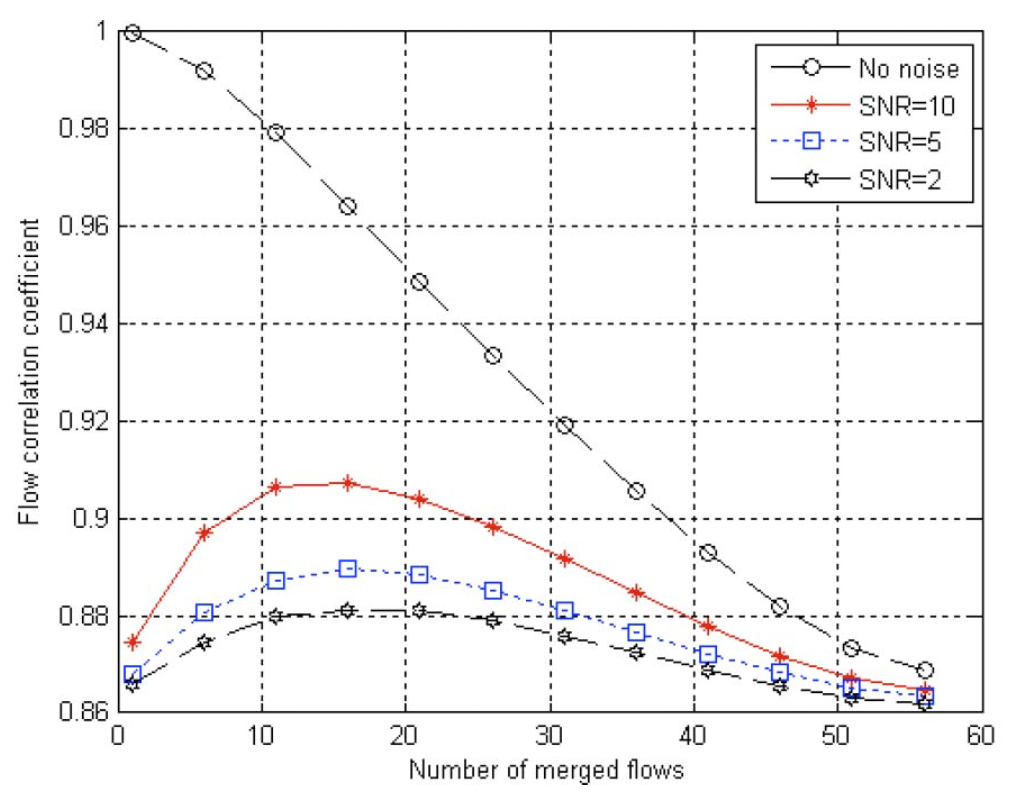
\includegraphics[width=0.9\textwidth,natwidth=1016,natheight=796]{figures/aggregate_attack.png}
\end{frame}

\section{Future Prospects and Challenges}

\begin{frame}
  \frametitle{Where is the Field Headed?} % subject to change

\end{frame}

\begin{frame}
  \frametitle{Where is the Competition Headed?} % subject to change

\end{frame}

\begin{frame}
  \frametitle{Questions?}
\end{frame}

\begin{frame}
  \frametitle{References}
  \begin{thebibliography}{}
    % use  \citep{zet96}, or \citet{blah}
  \bibitem[Shui Yu and Thapngam, T. and Jianwen Liu and Su Wei and
    Wanlei Zhou] _Shui Yu and Wanlei, J. et al. 2012, Parallel and
    Distributed Systems IEEE. Discriminating DDoS Attacks from Flash
    Crowds Using Flow Correlation Coefficient
  \bibitem[Byungha Choi and Kyungsan Cho] _Byungha Choi and Kyungsan
    Cho. 2012. Detection of Insider Attacks to the Web Server
  \bibitem[Barua, A. and Shahriar, H. and Zulkernine, M.] _Barua,
    A. and Shahriar, H. and Zulkernine, M. 2011, Software Reliability
    Engineering IEEE. Server Side Detection of Content Sniffing Attacks
  \end{thebibliography}
\end{frame}

\end{document}
